\chapter{System Design}
\label{chap:systemDesign}
%Intro to project
As explained in section \vref{sec:admin}, the Admin system is based on a single code base running on a LAMP stack. Which means we use Apache, MySQL and PHP for the system to operate. However the MySQL part is handled by another group, the WASTELAND group. The Admin system simply interface with the database through the API that the WASTELAND group makes. A description of the WASTELAND project can be read in section \vref{sub:wasteland}.\\
Given that the system is written in PHP, the product of this project will be a website. Which has the ability to manage users, pictograms and applications.\\
\\
This chapter will give an insight into the initial choices made by the Admin group at the beginning of the project. Choices such as, starting the project from scratch for the 3rd time, how to run PHP code on a Android device, and how we organize the source code.


\section{Starting from scratch}
%Why did we skip the old codebase
%What are we using now
Though there have been 3 \ac{giraf} administration projects before this one, the decission to create a completely new one came fairly easy.\\
The choice was made based on several problems with the two admin projects from the \ac{giraf} project year 2012. The projects was named Oasis and Savannah.\\
\\
Oasis was a system mainly concerned with constructing a database for the tablet, and every application run on the tablet. The administration part of this project did therefor not get far. It could more or less only display the information about users in the local database that it was constructed with.\\
\\
The Savannah admin interface got a little further than Oasis. However they too were also concerned with constructing a database, this time for the website version. It was supposed to be able to match that of the Oasis project. However this was not the case when the two projects was done. The database schemes did not match and was not able to syncronize. This lead to the start of the WASTELAND project.\\
The WASTELAND project was supposed to have been mainly about the synchronization of the two databases, but ended up having to start the database project from scratch because the available code from the Savannah project was outdated and that of Oasis was unusable as a central database setup.\\
By the same two reasons could the Admin project not be continued on from the Savannah or Oasis project. If we had chosen to continue on the Savannah and Oasis project, we would first of all have to get the Savannah code back up to date and then make both the Savannah and Oasis project complete, while making both ready for a new database implementation. This would also mean that it would be more difficult then necessary to maintain the Admin system when the project was finished. Since this would result in two entirely different code bases, one in Java and another in Java Servlet.\\
\\
All these reasons made the decision to start this project from scratch easy. Developing the system in PHP would make it possible to keep a single code base. And the time it would have taken to take Savannah and Oasis up to a state where they could both be worked on properly, both with a new DB and with their original features, would take at least the same time as it would to rewrite the system in a single code base.\\
\\
The next problem that this presents is that, PHP code is not normally something Android systems can interpret on their own. How we intend to solve this problem is what the next section is about.

\section{PHP on Android}
%PAW and why it didn't become anything
%PAW! Is the answer.\\
%PAW is an open source project
PAW stands for Pro Active Webfilter and is an application that makes it possible to run a website, written in PHP code on an Android device. This makes it possible, in combination with a web-browser for the user to use the Admin system without being online, which can be the case for the target group to use the \ac{giraf} system.\\
However we did not have the chance to implement this ourselves, since halfway through the project our tablet went haywire and was not fixed before the end of the project. This also meant that nearly nothing was finished in regard of this feature. Instead we focused on finishing the code base.

\section{Folder structure and other practical issues}
In this section we breifly explain the folder structure as well as why we chose to implement language support and use PHP and JavaScript as the coding languages.

\subsection{Folder Structure}
%The folder structure
When designing a system that is supposed to come with a high maintainability it is important to design a useable folder structure. The folder structure of the admin project can be seen in figure \ref{fig:folderStructure}.\\
\\

\begin{figure}[htbp]
        \centering
                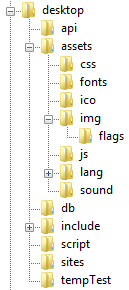
\includegraphics[width=0.25\textwidth]{images/folderStructure.png}
        \caption{The Code Folder Structure}
        \label{fig:folderStructure}
\end{figure}

\noindent{\textbf{desktop:} This is the main directory for the dekstop version. The reason for not having a single root directory is that there might be some variations between the desktop and the Android version of the system.}\\
\\
\textbf{api:} Is intended to contain API's that is not JavaScript or PHP code. And is empty as of the end of this project.\\
\\
\textbf{assets:} Contains every asset in the system. Images, JavaScript, sound, fonts, CSS and language files.\\
\\
\textbf{assets - css:} Contains the CSS files for the system.\\
\\
\textbf{assets - fonts:} Contains special fonts for the system.\\
\\
\textbf{assets - ico:} Contains the icon files for the system.\\
\\
\textbf{assets - img:} Contains the static image files for the system. Pictograms and Profile Images are loaded from the database.\\
\\
\textbf{assets - img - flags:} Contains images of flags, used for changing language.\\
\\
\textbf{assets - js:} Contains all JavaScript in the system, files are named as they fit to PHP files, as far as this is possible.\\
\\
\textbf{assets - lang:} Contains all language files for the system. Each webpage and some JavaScripts, have their own language sub-folder . Right now they contain English and Danish language files.\\
\\
\textbf{assets - sound:} Contains all static sound files for the system. Sounds for Pictograms are loaded from the database.\\
\\
\textbf{db:} Contains the database files. All active database functions is stored in the file ``new.db.php''\\
\\
\textbf{include:} Contains any JavaScript or PHP code that is not developed by the Admin project, that is included in the system.\\
\\
\textbf{script:} Contains PHP scripts that does not display anything, but rather works to execute some function. Such as changing a profile image.\\
\\
\textbf{sites:} Contains .html and .php files that corresponds to a webpage on the website.\\
\\
\textbf{tempTest:} A folder for any need of generating files during development.

\subsection{PHP and JavaScript}
%Why PHP and JavaScript
As already mentioned in this chapter we chose to use PHP as the backend language. And in order to make some more advanced user interface we decided to use JavaScript, HTML and CSS as frontend language.\\
We chose to use PHP because most of the Admin group already had experience with the language, and also because we found PAW that would make it possible to execute the PHP code on the tablet.\\
Also another bonus, that was not considered much when we made the choice, is that PHP is natively able to work with JSON objects which is how we communicate with the database API.\\
\\
JavaScript, HTML and CSS was chosen as frontend because of the product being a website, for which there is no real alternative.

\subsection{Language Support}
%Language Support
It was in the beginning of the project suggested that the system could be operated in multiple languages, as a start in Danish and English. This was suggested by the semester coordinator. The admin group thought, if this was to implemented at any point, it should be in the start of the system, which meant we would have to implement it into our system.\\
The way it is implemented is much like it is in Android applications, and can be read in further detail in \vref{sec:languageSupport}.\\
\\
The reader should now have an understanding of the most basic decisions of the Admin project, and be able to navigate in our system.\\
The next chapter will go through the project progress, followed by the project's problem statement.
